\documentclass[10pt,a4paper]{report}

\usepackage[utf8]{inputenc}
\usepackage[T2A]{fontenc}
\usepackage[english, russian]{babel}
\usepackage{hyperref}
\usepackage[table]{xcolor}
\usepackage{mathtools}
\hypersetup{
    colorlinks=true,
    linkcolor=blue,
    filecolor=magenta,  
    citecolor = blue,
    urlcolor=blue,
    pdftitle={Overleaf Example},
    pdfpagemode=FullScreen,
    }
\urlstyle{same}
\usepackage{sectsty}
\usepackage[sorting = none]{biblatex}
\addbibresource{bib.bib}
\usepackage{url}
\usepackage{amssymb}

\newcolumntype{s}{>{\columncolor[HTML]{c9a0dc}} l}
\renewcommand{\arraystretch}{1.3}
\setlength{\arrayrulewidth}{0.5mm}
\usepackage{graphicx}
\usepackage{array}
\usepackage{wrapfig}
\usepackage{caption}
\usepackage{subcaption}
\usepackage{blindtext}
\usepackage{quotchap}
\usepackage{csquotes}
\usepackage{multicol}
\usepackage{diagbox}

% \title{
% \large
% <<Национальный исследовательский университет>> 

% <<Высшая школа экономики>>
% \vspace{4cm}

% \textbf{
% \Large
% Сравнение образов фестиваля «Burning Man» в произведениях массовой культуры}
% \vspace{5cm}
% }
% \author{
% \vbox{\hfill\vbox{\hbox{\textit{Kовалевская Виктория Владимировна}}}}
% \vspace{4cm}
% }
% \date{2022}

\begin{document}

% \maketitle

\begin{titlepage}

\center 
 
\textsc{\large Федеральное госудраственное автономное образовательное учреждение высшего образования}\\[1.5cm]
\textsc{\Large \textbf{<<Национальный Исследовательский Университет Высшая Школа Экономики>>}}\\[4.4cm]

\huge \bfseries Сравнение образов фестиваля «Burning Man» в произведениях массовой культуры\\[1.4cm] 

\begin{flushleft} 
\normalsize
\emph{Выполнил:}\\
Студент группы БПМИ2111 \\
Ковалевская Виктория Владимировна \\[2cm]
\end{flushleft} 


\includegraphics[width=3.5cm, height=3.5cm]{images/logo.png}\\[1.5cm]

\textsc{\large Москва 2022}

\end{titlepage}

\begin{abstract}
Праздник как специфический аспект деятельности человека 
существует с момента зарождения культуры и наблюдается на
всех стадиях 
развития человеческой цивилизации, в любых географических или
экономических условиях\footnote{Николаева П. Фестиваль как этап эволюции
праздничной культуры // Культурная жизнь Юга России. 2008. №2 (27). С. 144-146.}.
В XIII веке возникает понятие «фестиваль»
(фр. festival; от лат. festivus — «праздничный»)\footnote{Фасмер М. 
Этимологический словарь русского языка / Пер. с нем. под ред. Б.А. Ларина. М.:
Прогресс, 1986.}. В современных 
социокультурных условиях это наиболее востребованный способ 
проведения массовых мероприятий с целью показа лучших достижений
искусства: музыкального, театрального, кино и т.п.\footnote{Там же. С. 144.}
Фестивали
занимают определенное место в обществе: в них участвует большое 
количество людей, на них обращают свое внимание СМИ, про них пишут 
книги и снимают фильмы. Один из таких фестивалей заинтересовал и 
меня.
\end{abstract}

\tableofcontents
\begin{savequote}[45mm]
Do not wait; the time will never be 'just right.' 
Start where you stand, and work with whatever tools 
you may have at your command, and better tools will 
be found as you go along.
\qauthor{George Herbert}
\end{savequote}

\chapter{Введение}

% \addcontentsline{toc}{subsection}{Рисунок 1}
\begin{wrapfigure}{l}{0.50\textwidth}
    \centering   
    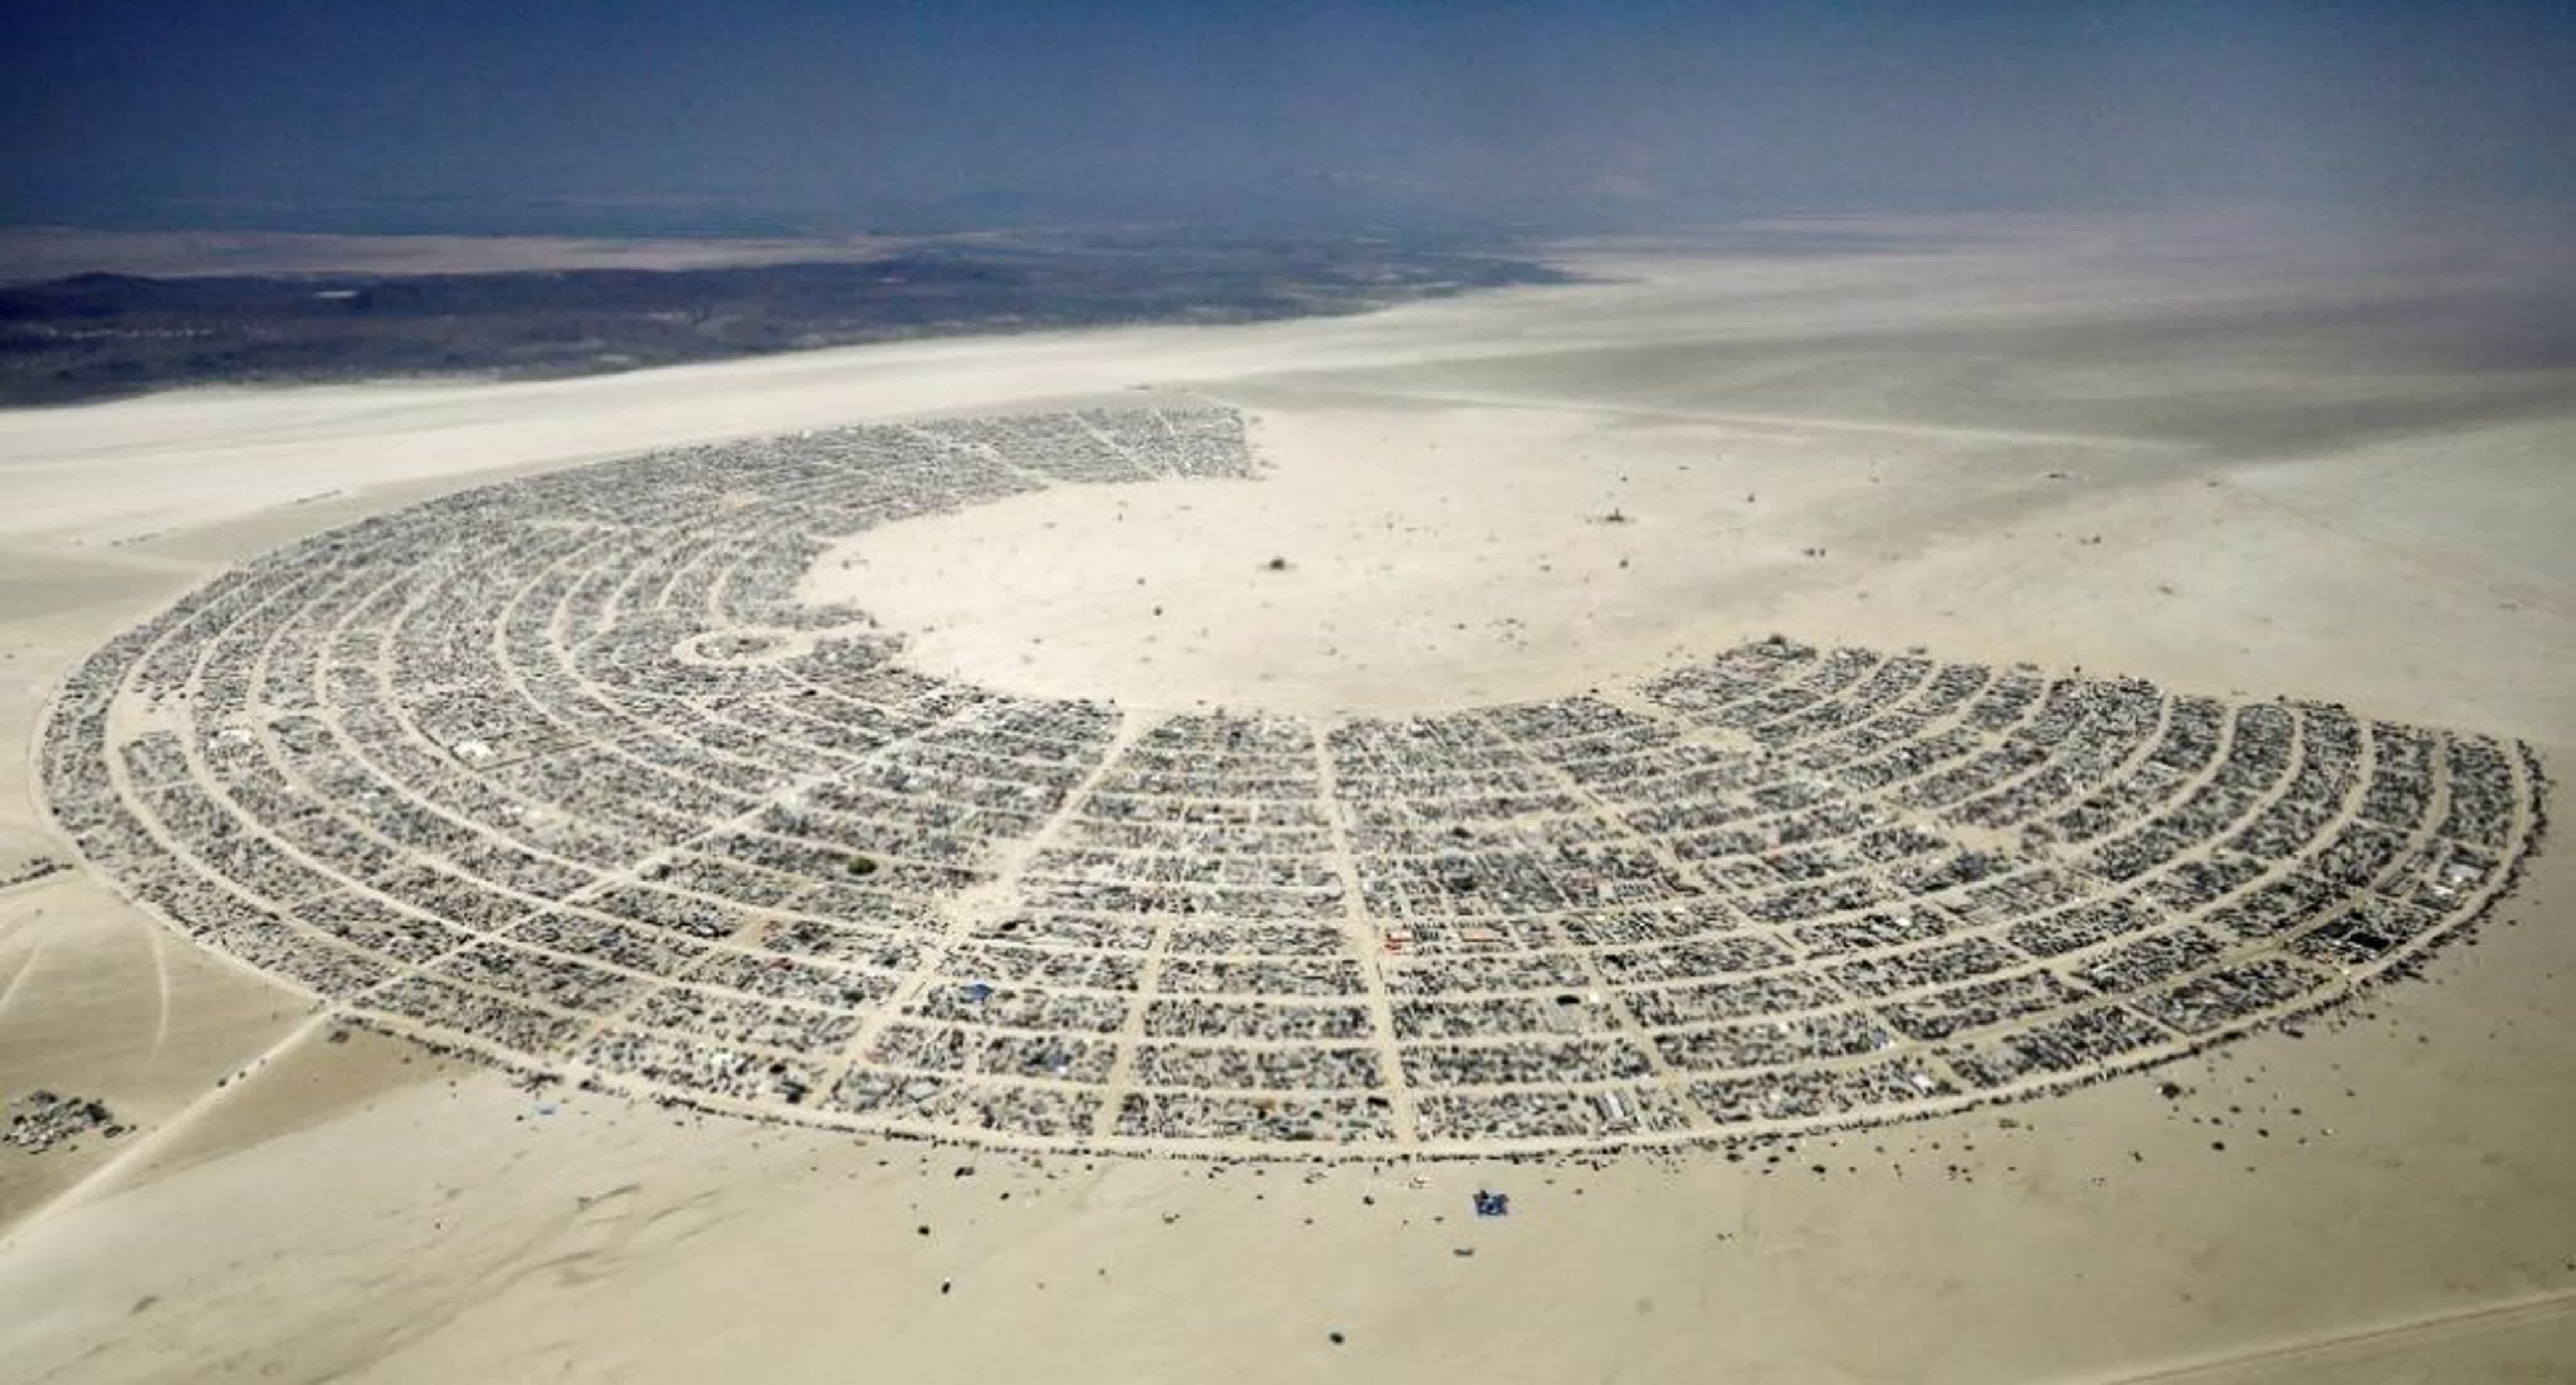
\includegraphics[width=0.50\textwidth]{images/burningman1.jpg}
    \caption{Вид на Burning Man с высоты птичьего полета}
    \label{picture:1}
\end{wrapfigure}

«Burning Man» - фестиваль со своей уникальной атмосферой творчества, свободы и самовыражения~\cite{gilmore2005afterburn}. 
Как и любой другой 
фестиваль, он дает возможность ведения
культурного диалога и генерирования 

% \addcontentsline{toc}{subsection}{Рисунок 2}
\begin{wrapfigure}{r}{0.50\textwidth}
    \centering   
    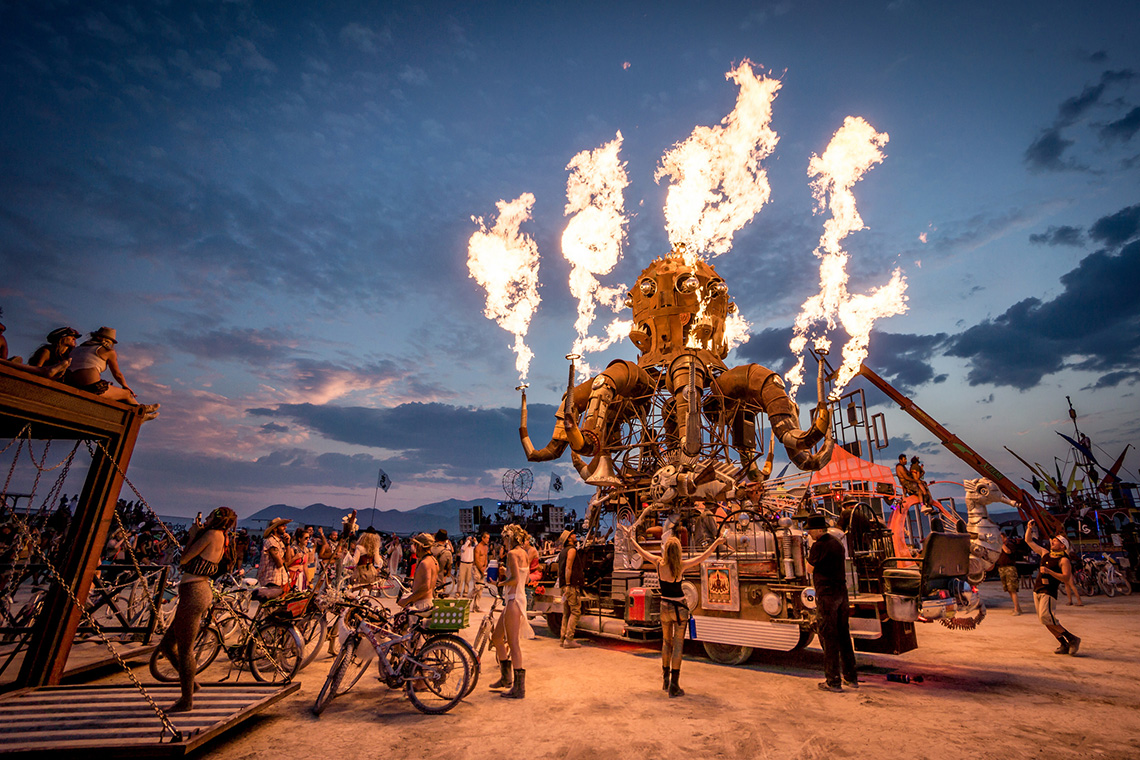
\includegraphics[width=0.50\textwidth]{images/burningman2.jpg}
    \caption{Одна из инсталляций}
    \label{picture:2}
\end{wrapfigure}

нового вида
искусства\footnote{Тихомирова Г.
Фестиваль как форма социально-культурной деятельности // Вестник
Таганрогского
института имени А.П. Чехова. 2016. С. 244.}. 
Однако главной ценностью «Burning Man» является его утопическая система
человеческих взаимоотношений. Данное событие - эксперимент по созданию
сообщества, полагающегося только на себя. 
Тысячи людей участвуют в нем и,
благодаря совместным усилиям, создают город посреди пустыни, где каждый
помогает друг другу и не просит ничего взамен, что редко
встретишь в современном мире.

Таким образом, у меня возникло желание более детально изучить фестиваль-
феномен «Burning Man», не принимая в нем непосредственного участия.

Цель данной работы - исследовать, как менялось представление образа фестиваля
«Burning Man» в произведениях массовой культуры с 1995 по 2017 годы.

Для достижения цели исследования будет использоваться метод контент-анализа, 
который предполагает работу с большим объемом визуального
материала.
\\
\\
Стоит выделить следующие задачи исследования:

\begin{itemize}
  \item Изучение основных механизмов, которые используются в контент-
  аналитическом методе;
  \item Изучение истории фестиваля «Burning Man» с момента его возникновения до
  наших дней;
  \item Контент-анализ выбранных произведений массовой культуры;
  \item Описание результатов, которые будут получены при сравнении образов 
  фестиваля «Burning Man».
\end{itemize}

\chapter{Теоретическая часть}
\section{История фестиваля <<Burning Man>>}

«Burning Man» - ежегодное мероприятие, которое проводится
в западной части Соединенных Штатов Америки в пустыне
Блэк Рок штата Невада. Особенность~\cite{николаева2008фестиваль} фестиваля заключена в
традициях и культуре, которые формировались и развивались
на протяжении всей истории «Burning Man».

В 1986 году два друга Ларри Харви и Джерри Джеймс
собрались на Бейкер-Бич в Сан-Франциско и построили
деревянного человека в восемь футов ($2,43$ м). Их целью
было получить удовольствие, поэтому они решили сжечь эту
статую на закате во время летнего солнцестояния. Однако
друзья не предполагали, что пламя привлечет других людей,
тоже искавших веселья. Поэтому 22 июня 1986 года тридцать
пять человек договорились между собой повторить через год
поджог деревянного человека на Бейкер-Бич. Так зародился
фестиваль «Burning Man»\footnote{Gilmore L., Van Proyen
M. Afterburn: reflections on burning man. New Mexico: 
University of New Mexico Press, 2005. P. 6.}.

Следующим важным этапом в истории «Burning Man» является
«Zone trip» (рус. «Зональный переезд»). К 1990 году
количество участников выросло до трехсот пятидесяти
человек, что начало приносить дискомфорт людям, которые
жили рядом с Бейкер-Бич. В результате федеральная полиция
настояла на выборе другого места для поджога человека уже
в сорок футов. Харви и остальные участники фестиваля
вступили в «The San Francisco Cacophony Society»
(«объединение людей, которые ищут новые впечатления за
пределами привычного общества»), после чего вместе с
какофонистами Майклом Микель и Джоном Лоу организовали
переезд в пустыню Блэк Рок во время выходных по случаю
американского праздника Дня труда. Так зародилась
традиция собираться на фестивале «Burning Man» с
последнего воскресенья августа по первый понедельник
сентября в пустыне Блэк Рок штата Невада, которая
является частью высохшего доисторического озера Лаонтан.

Переломным моментом в истории «Burning Man» является 1996 год,
когда у восьми тысяч участников появилась специальная карта с
обозначениями. Тогда же фестиваль приобрел официальную тему, в
которую были включены несколько объектов искусства - инсталляции,
созданные лично участниками. Так возник город под названием Блэк
Рок Сити со своими культурными особенностями и временными
жителями . В 2018 году их число превысило семьдесят тысяч.
Участники гордо называют себя «burners».

Фестиваль «Burning Man»~\cite{ньюман1998неопросные}
имеет десять заповедей, которые необходимо знать, прежде чем посещать пустынный
город :

\begin{enumerate}
\item Радикальное включение. Каждый участник может добровольно
включиться в те или иные процессы фестиваля, и возраст не будет
являться преградой.
\item Дарение. Задача «Burning Man» - научить человека относиться
к вещам проще и безвозмездно отдавать их. Ценность денег здесь
почти отсутствует – единственное, что можно купить на фестивале – 
это кофе и лед. Доходы передаются местным школам.
\item Декоммодификация. Отказ от коммерциализации за счет
спонсоров и рекламы.
\item Радикальная самодостаточность. Ответственность за свою
безопасность. Стоит надеяться только на себя. На официальном
сайте~\url{https://burningman.org} предоставлен гид по выживанию в
пустыне. Также ответственность за безопасность других. Не стоит
делать того, что может навредить людям вокруг.
\item Радикальное самовыражение. Каждый участник пытается
проявить свою индивидуальность. Особенно в искусстве: костюмы,
художественные инсталляции, «мутант-кары» («мутированные» машины,
которые создаются непосредственно участниками), танцы, пение,
чтение стихов и т.д. Существует также специальная зона, которая
называется «Center Camp», где люди показывают свои сценические
выступления.
\item Общественные усилия. Пустынный город невозможно построить
без слаженной работы. Волонтерская деятельность на фестивале
также приветствуется.
\item Гражданская ответственность. На фестивале «Burning Man» 
действуют законы США и штата Невада.
\item Не оставлять следа. После окончания фестиваля пустыня
должна вернуться в свое первоначальное состояние.
\item Участие. Экстремальные условия жизни в пустыне дают каждому
участнику осознание того, что он может стать полезным для других.
\item Здесь и сейчас. На фестивале «Burning Man» участники
доверяют случаю и живут моментом.
\end{enumerate}

\section{Материалы исследования}

Прежде чем приступить к основной части исследования, нужно
обозначить, с какими произведениями массовой культуры я буду
работать.

«Burning Man» является относительно новым фестивалем, о котором с
каждым годом узнают все больше и больше людей. Таким образом,
можно зафиксировать всего лишь пять упоминаний «Burning Man» в
произведениях массовой культуры с 1995 по 2017 года:

\begin{enumerate}
\item Мультипликационный сериал «Симпсоны» (1995);
    \begin{enumerate}
        \item Season 6
        \begin{enumerate}
            \item Episode 18
        \end{enumerate}
    \end{enumerate}
\item Сериал «Малкольм в центре внимания» (2005);

\item Рассказ «Тусовщик» автора Чака Паланика (2015);

\item Компьютерная игра «Watch Dogs 2» (2016);

\item Художественный фильм «Девушка из песни» (2017).

\end{enumerate}

\begin{figure}
\centering
     \begin{subfigure}[b]{0.3\textwidth}
         \label{pic1} 
         \centering
         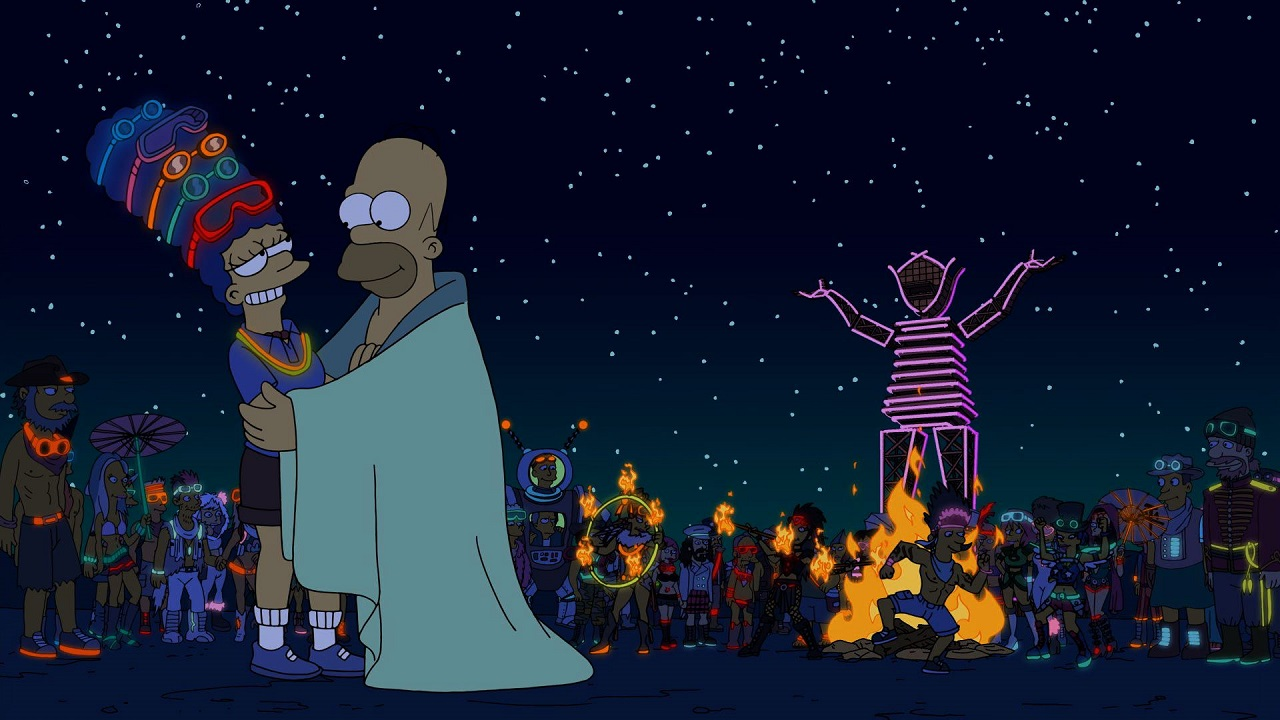
\includegraphics[width=\textwidth]{images/simpsons1.jpg}
         \caption{Симпсоны}
     \end{subfigure}
     \hfill
     \begin{subfigure}[b]{0.3\textwidth}
         \label{pic2}
         \centering
         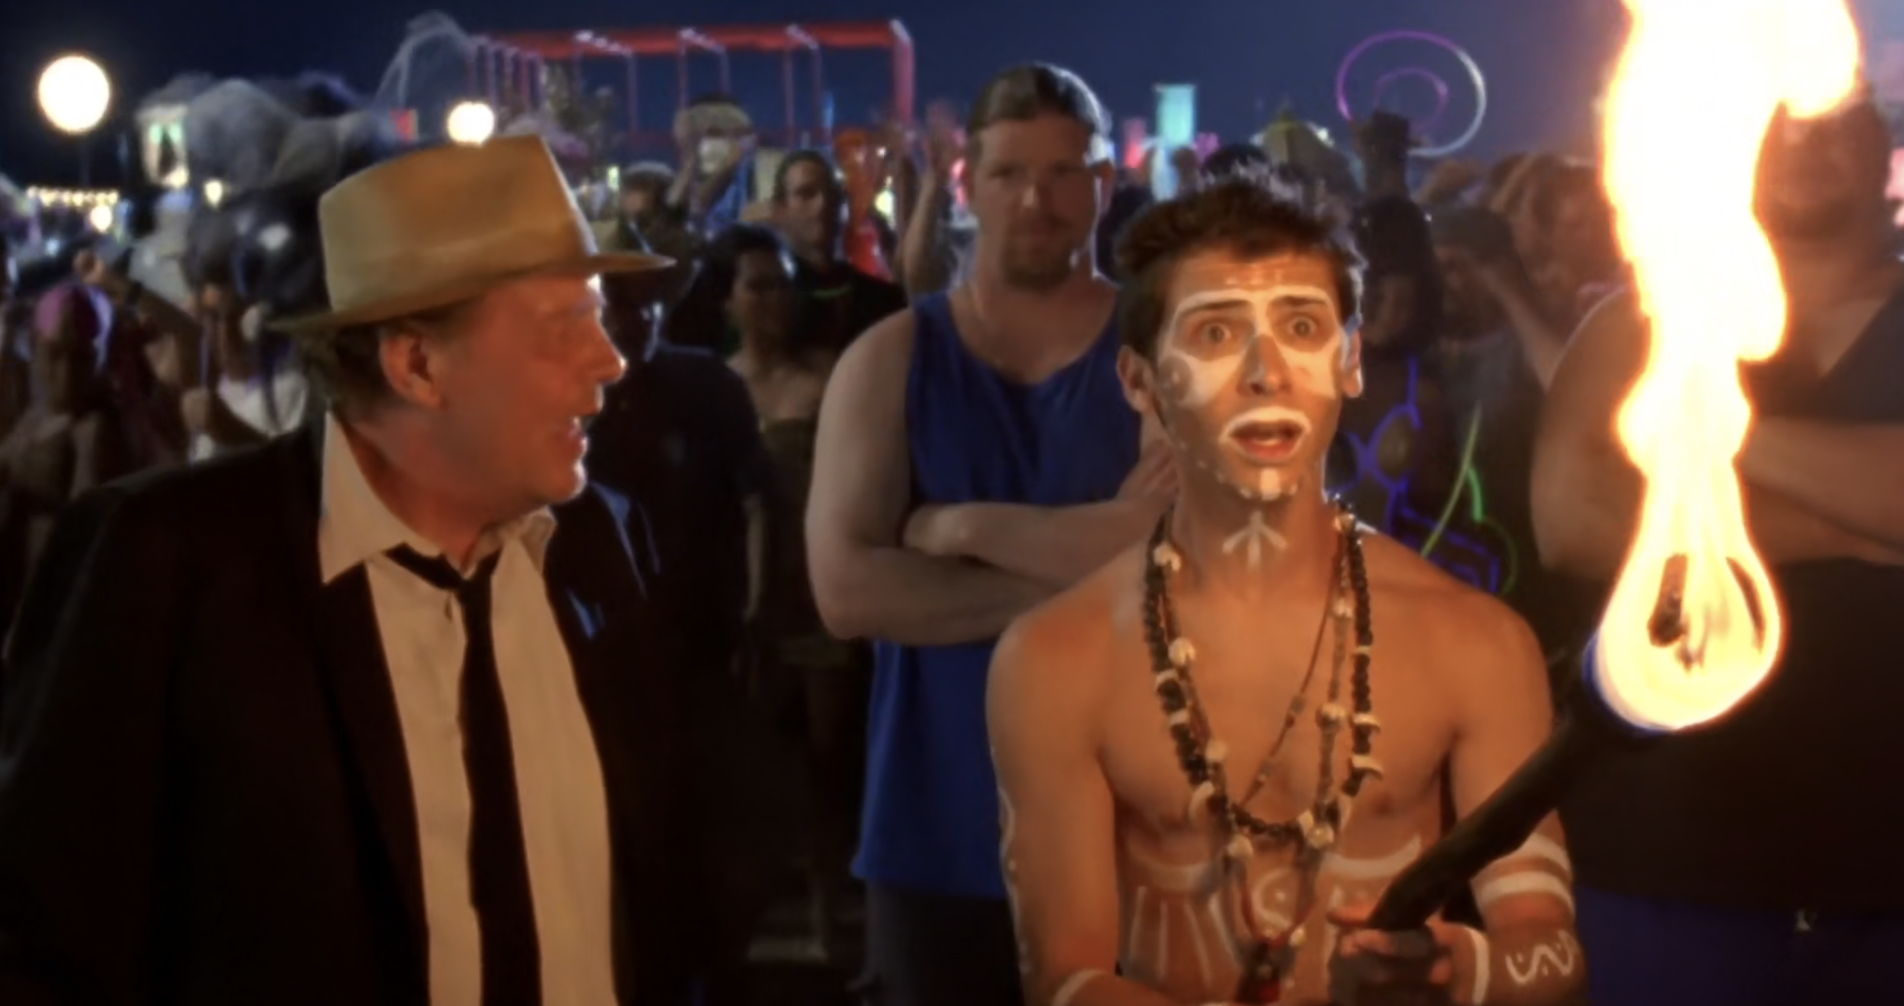
\includegraphics[width=\textwidth]{images/malcolm2.jpg}
         \caption{Малкольм в центре внимания}
     \end{subfigure}
     \hfill
     \begin{subfigure}[b]{0.3\textwidth}
         \label{pic3}
         \centering
         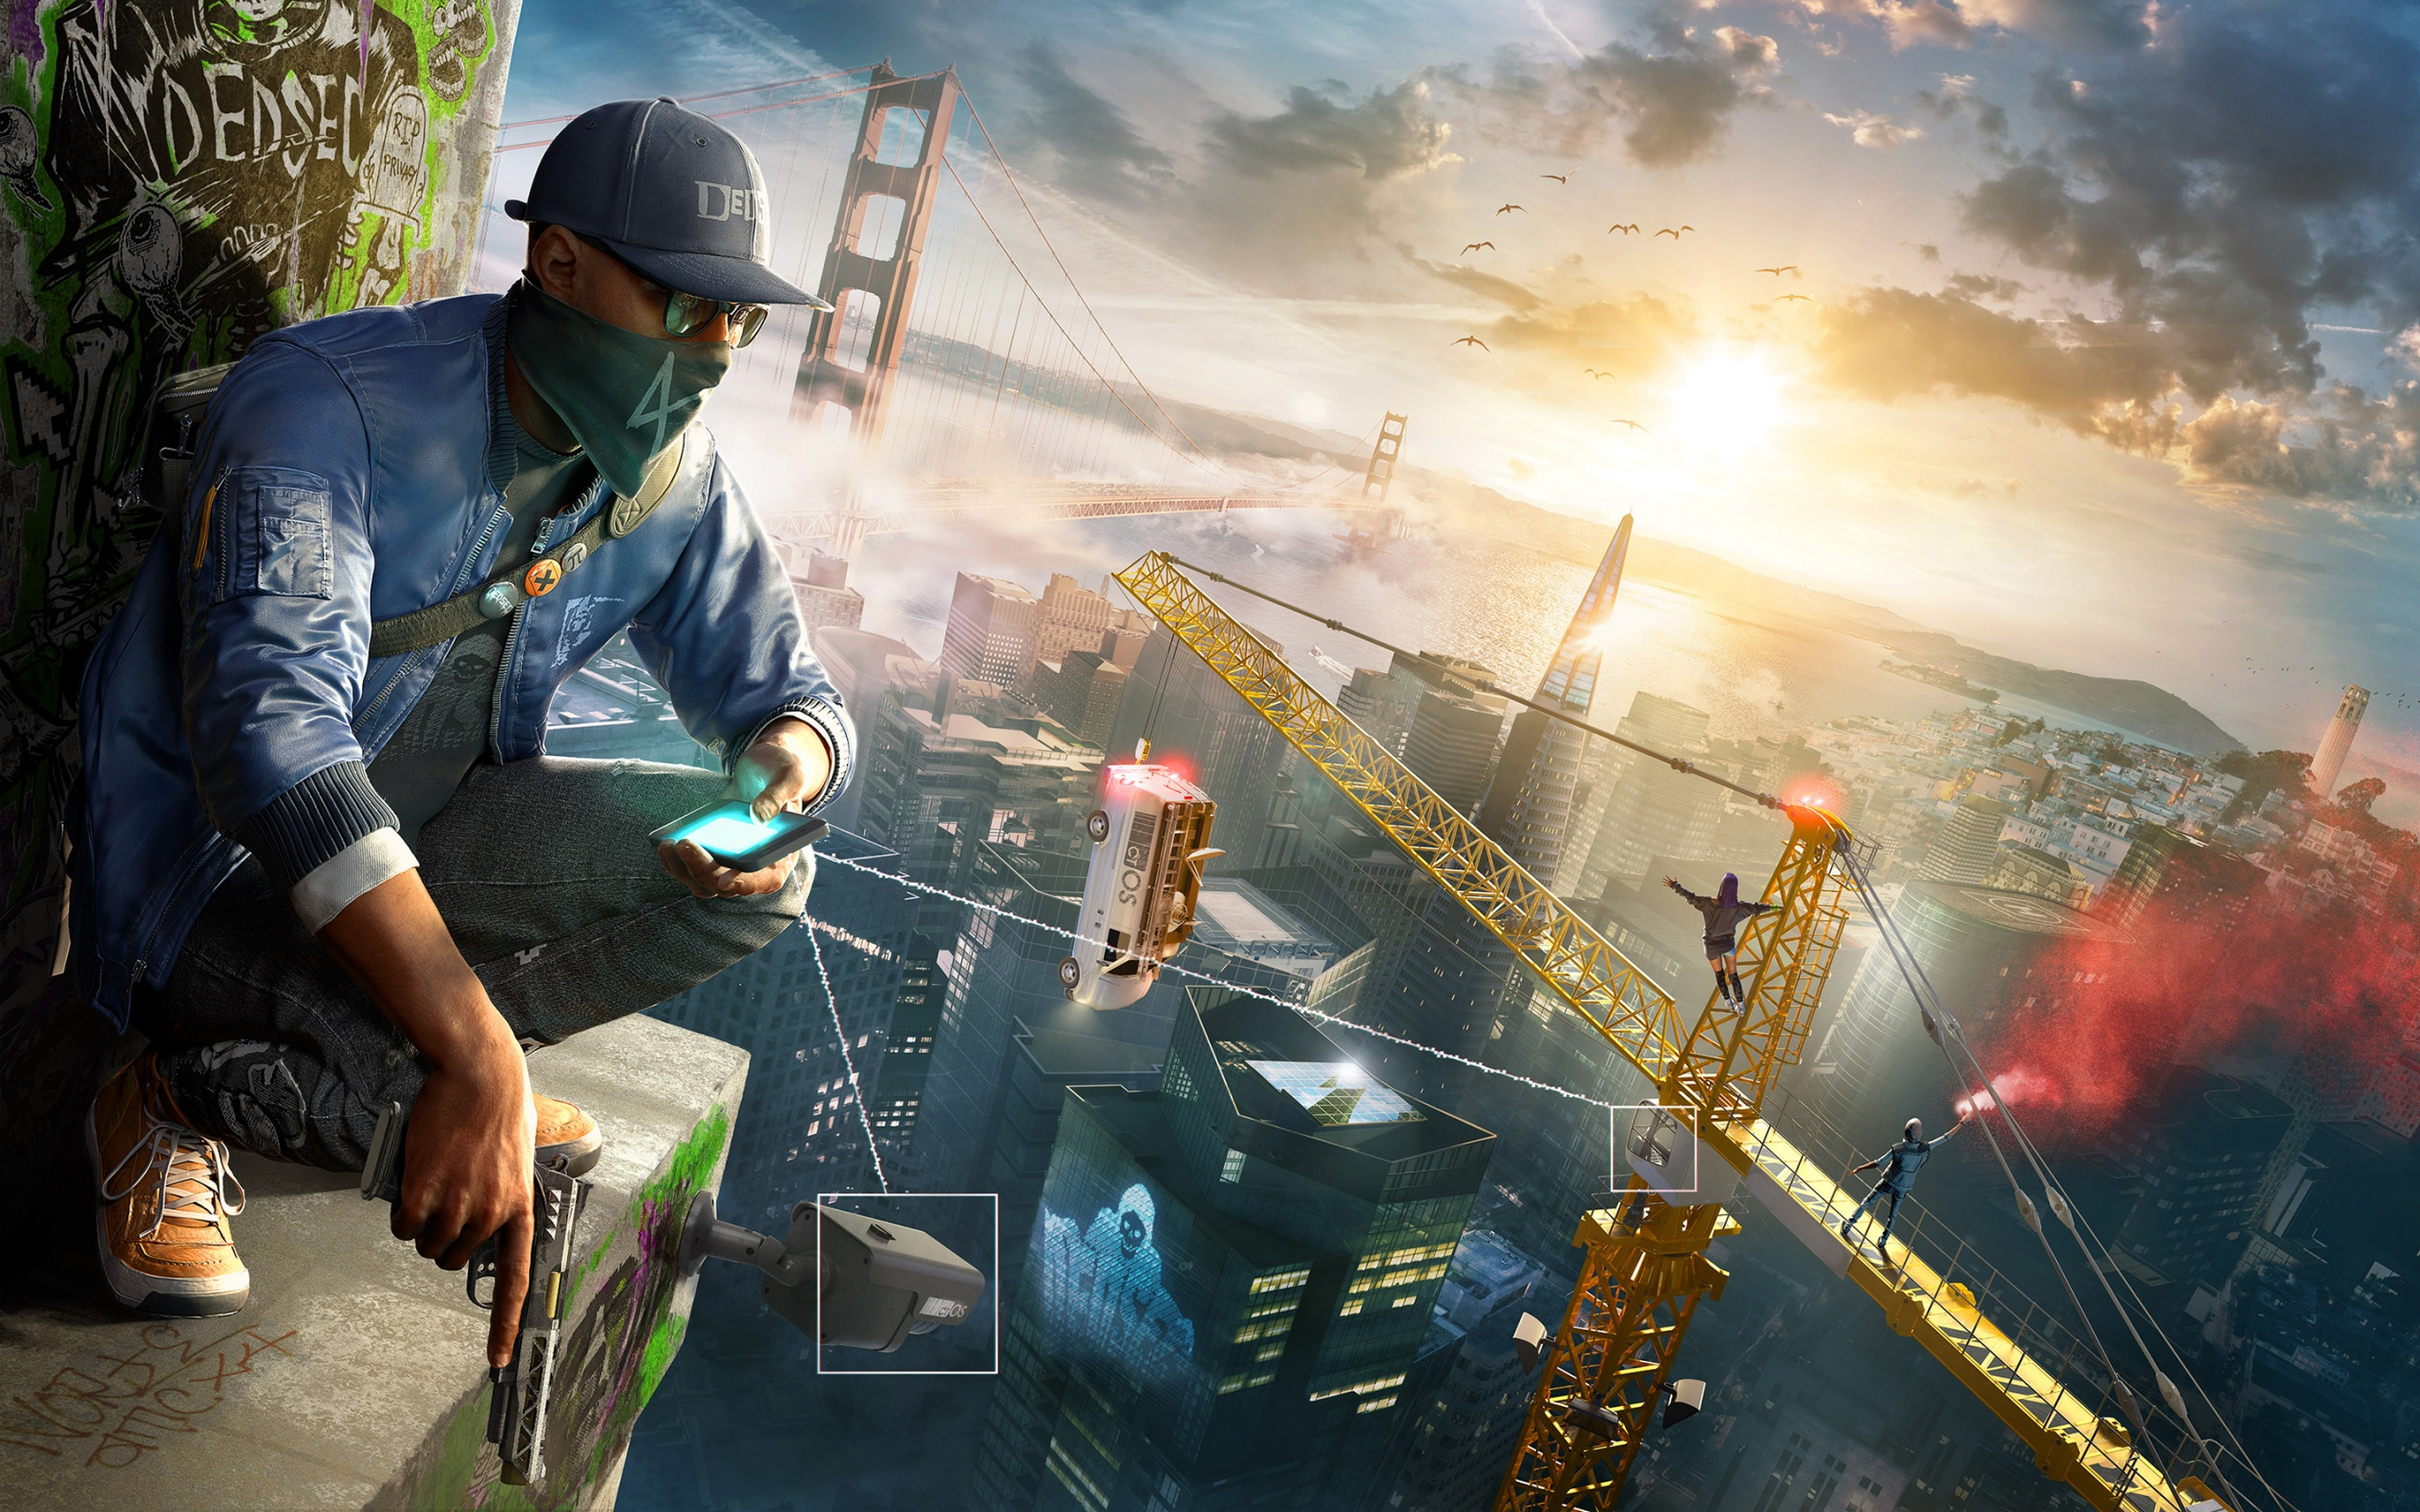
\includegraphics[width=\textwidth]{images/watchdogs2.jpeg}
         \caption{игра «Watch Dogs 2»}
     \end{subfigure}
     \hfill
     \begin{subfigure}[b]{0.3\textwidth}
         \label{pic4}
         \centering
         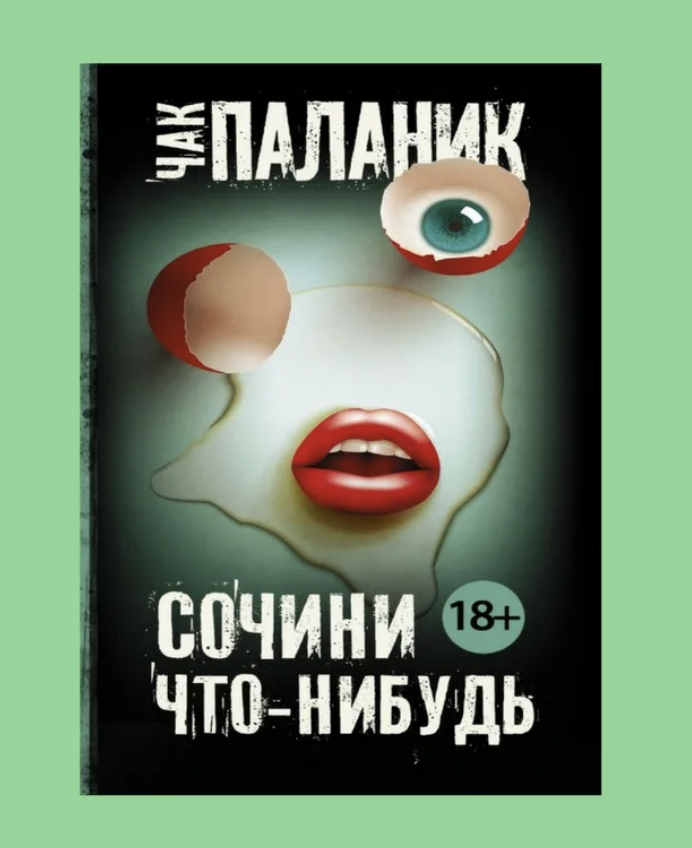
\includegraphics[width=\textwidth]{images/тусовщик.png}
         \caption{Рассказ «Тусовщик»}
     \end{subfigure}
     \begin{subfigure}[b]{0.3\textwidth}
         \label{pic5}
         \centering
         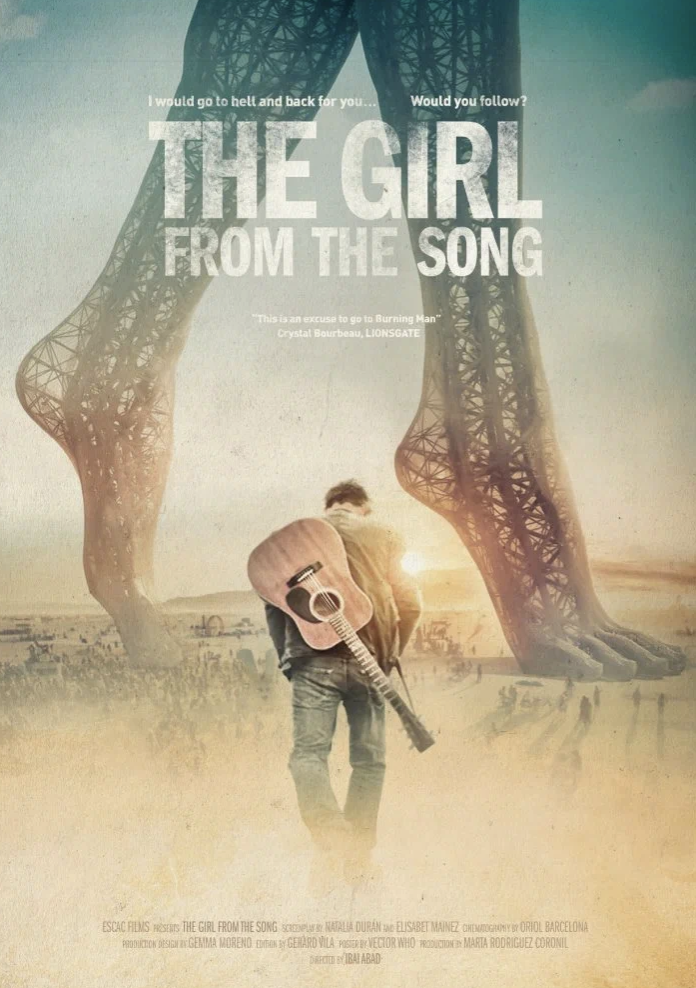
\includegraphics[height = 4.5cm, width=\textwidth]{images/девушкаизпесни.png}
         \caption{«Девушка из песни»}
     \end{subfigure}
     \caption{Произведения}
\end{figure}

Становится понятно, что исследование предполагает работу с
разнородными материалами. Делать выборку наиболее подходящих
произведений массовой культуры я считаю неразумным, так как из-за
маленького количества материала будет невозможно полностью
ответить на ключевой вопрос: 
\begin{displayquote}
«Как менялось представление образа
фестиваля~\cite{ньюман1998неопросные} «Burning Man» в произведениях массовой
культуры?»
\end{displayquote}
Поэтому я буду рассматривать все пять произведений культуры, где
упоминается «Burning Man», учитывая при этом их видовые и
жанровые особенности. Такой подход поможет сделать исследование
качественным и объективным.

Стоит также отметить, что в качестве материалов исследовательской
работы я намеренно исключила такие произведения массовой
культуры, как выпуски или блоги от первого лица с видеохостинга
«YouTube». В подобных видео фестиваль «Burning Man» является
ключевой фигурой для повествования и описания, что больше похоже
на документальный жанр. В пяти выбранных произведениях массовой 
культуры фестиваль является лишь вторым планом – подходящей
локацией для действий в сериале, мультсериале, фильме, рассказе
или игре.

\subsection{Приложение 1}

С основными сведениями о материалах исследования можно
ознакомиться ниже в таблице\footnote{Данные были получены из электронных
ресурсов \url{https://www.kinopoisk.ru} и \url{https://ru.wikipedia.org}}.

\begin{table}[h!]
\centering
\begin{tabular}{|s !{} c !{} c |}
 \arrayrulecolor[HTML]{a00040}\hline
 \textbf{Название} & \cellcolor[HTML]{f5deb3}\textbf{Симпсоны} & \cellcolor[HTML]{ffbf94}\textbf{Малкольм в центре внимания} \\
 \hline
 \textbf{Год} & \cellcolor[HTML]{ffbf94}1995 & \cellcolor[HTML]{f5deb3}2005 \\
 \hline
 \textbf{Вид} & \cellcolor[HTML]{f5deb3}Мультипликационный сериал  & \cellcolor[HTML]{ffbf94}Сериал \\
 \hline
 \textbf{Жанр} & \cellcolor[HTML]{ffbf94}Комедия, ситком, сатира, черный юмор & \cellcolor[HTML]{f5deb3}Комедия, ситком, семейный \\
 \hline
 \textbf{Страна} & \cellcolor[HTML]{f5deb3}США & \cellcolor[HTML]{ffbf94}США \\
 \hline
 \textbf{Студия} & \cellcolor[HTML]{ffbf94}20th Century Fox Television & \cellcolor[HTML]{f5deb3}20th Century Fox Television \\
 \hline
 \textbf{Режиссер} & \cellcolor[HTML]{f5deb3}Мэтт Грейнинг & \cellcolor[HTML]{ffbf94}Тодд Холлэнд \\
 \hline
 \textbf{Длина} & \cellcolor[HTML]{ffbf94}21 мин & \cellcolor[HTML]{f5deb3}20 мин \\
 \hline
\end{tabular}
\caption{Приложение 1}
\label{table:1}
\end{table}

\begin{table}[h!]
\centering
\begin{tabular}{c | c | c}
\backslashbox{фильм}{смотреть ли} & Да & Нет \\
\hline
Симсоны & \checkmark & -- \\
\hline
Малкольм в центре внимания & --  & \checkmark
\end{tabular}
\caption{Личные рекомендации}
\end{table}

\chapter{Основная часть}

\section{«Симпсоны» (1995)}

«Симпсоны» — это американский мультипликационный сериал режиссера Мэтта
Грейнинга в жанре ситуационной комедии, который выпускается с 1989 года.
Каждая серия показывает жизнь семьи Симпсонов и других жителей
вымышленного города Спрингфилд. Особенность сериала заключается в
высмеивании стереотипов и ситуаций, касающихся семейной жизни, школы,
мировой культуры, а также политики и религии.

В 1995 году была выпущена седьмая серия двадцать девятого сезона под
названием «Blazed and confused» («Сражен и запутан»). Значительная часть
действий серии происходит на фестивале «Burning Man» \ref{picture:1}. 
Сюжетная линия разворачивается вокруг семьи Симпсонов, которые отправляются на праздник
«Blazing Guy», проходящий где-то в пустыне, и вокруг Барта Симпсона –
старшего ребенка в семье – и его школьного друга Милхауса, которые
пытаются дискредитировать своего нового учителя Мистера Лассона, также
отправившегося на фестиваль.

\section{«Малкольм в центре внимания» (2005)}

«Малкольм в центре внимания» - американский комедийный сериал режиссера
Тодда Холлэнда, который выпускался с 2000 по 2006 года. В нем
рассказывается про юного гения Малкольма и его большую семью, которая
живет под одной крышей. Цель каждой серии – с иронией описать
взаимоотношения пятерых братьев и их родителей, а также показать другие
социальные проблемы в обществе.

В 2005 году была выпущена первая серия седьмого сезона под названием
«Burning Man». Сюжетная линия разворачивается вокруг двух братьев,
Малкольма и Риза, которые собираются тайно поехать на фестиваль в
пустыне. Их останавливают родители, но Малкольму удается успокоить и даже
заинтересовать праздником маму с папой. В итоге вся семья решает поехать
на «Burning Man», где происходит много интересных событий.

\subsection{Приложение 2}

\begin{table}[h!]
  \centering
  \begin{tabular}{  m{55mm} | m{55mm} }
  \centering
    \cellcolor[HTML]{f297ff}\textbf{Симпсоны} & \cellcolor[HTML]{b3fcff}\textbf{Малкольм в центре внимания}\\
    \hline
    \\
    \begin{minipage}{.3\textwidth}
      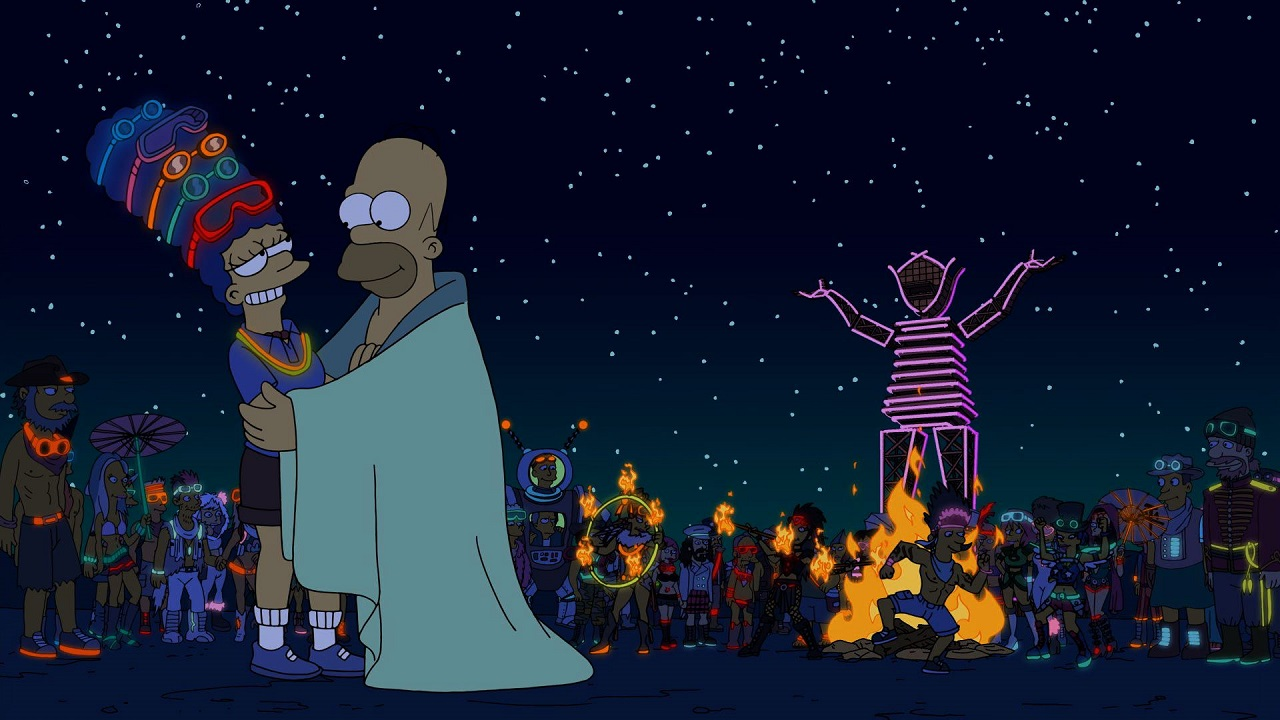
\includegraphics[height=30mm]{images/simpsons1.jpg}
    \end{minipage}
    \vspace{\baselineskip}
    \begin{minipage}{.3\textwidth}
      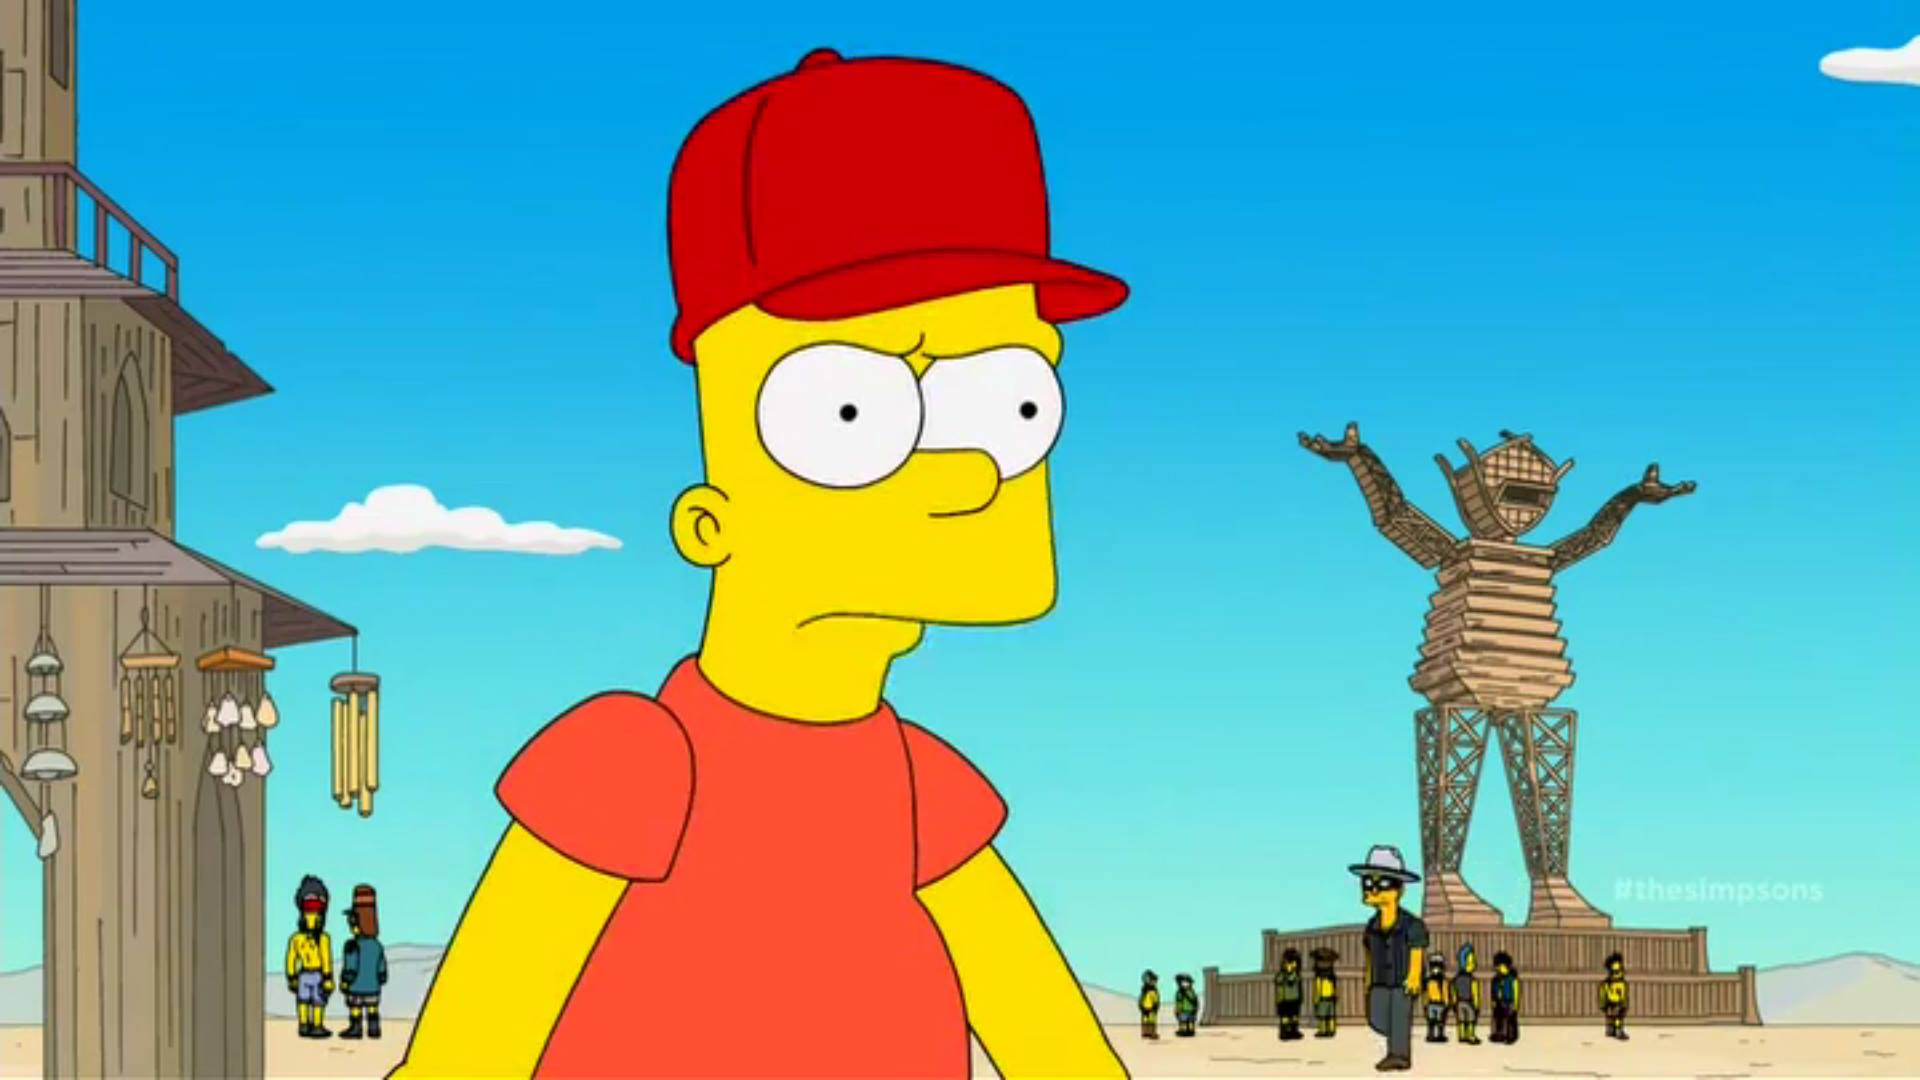
\includegraphics[height=30mm]{images/simpsons2.jpg}
    \end{minipage}
    &
    \begin{minipage}{.3\textwidth}
      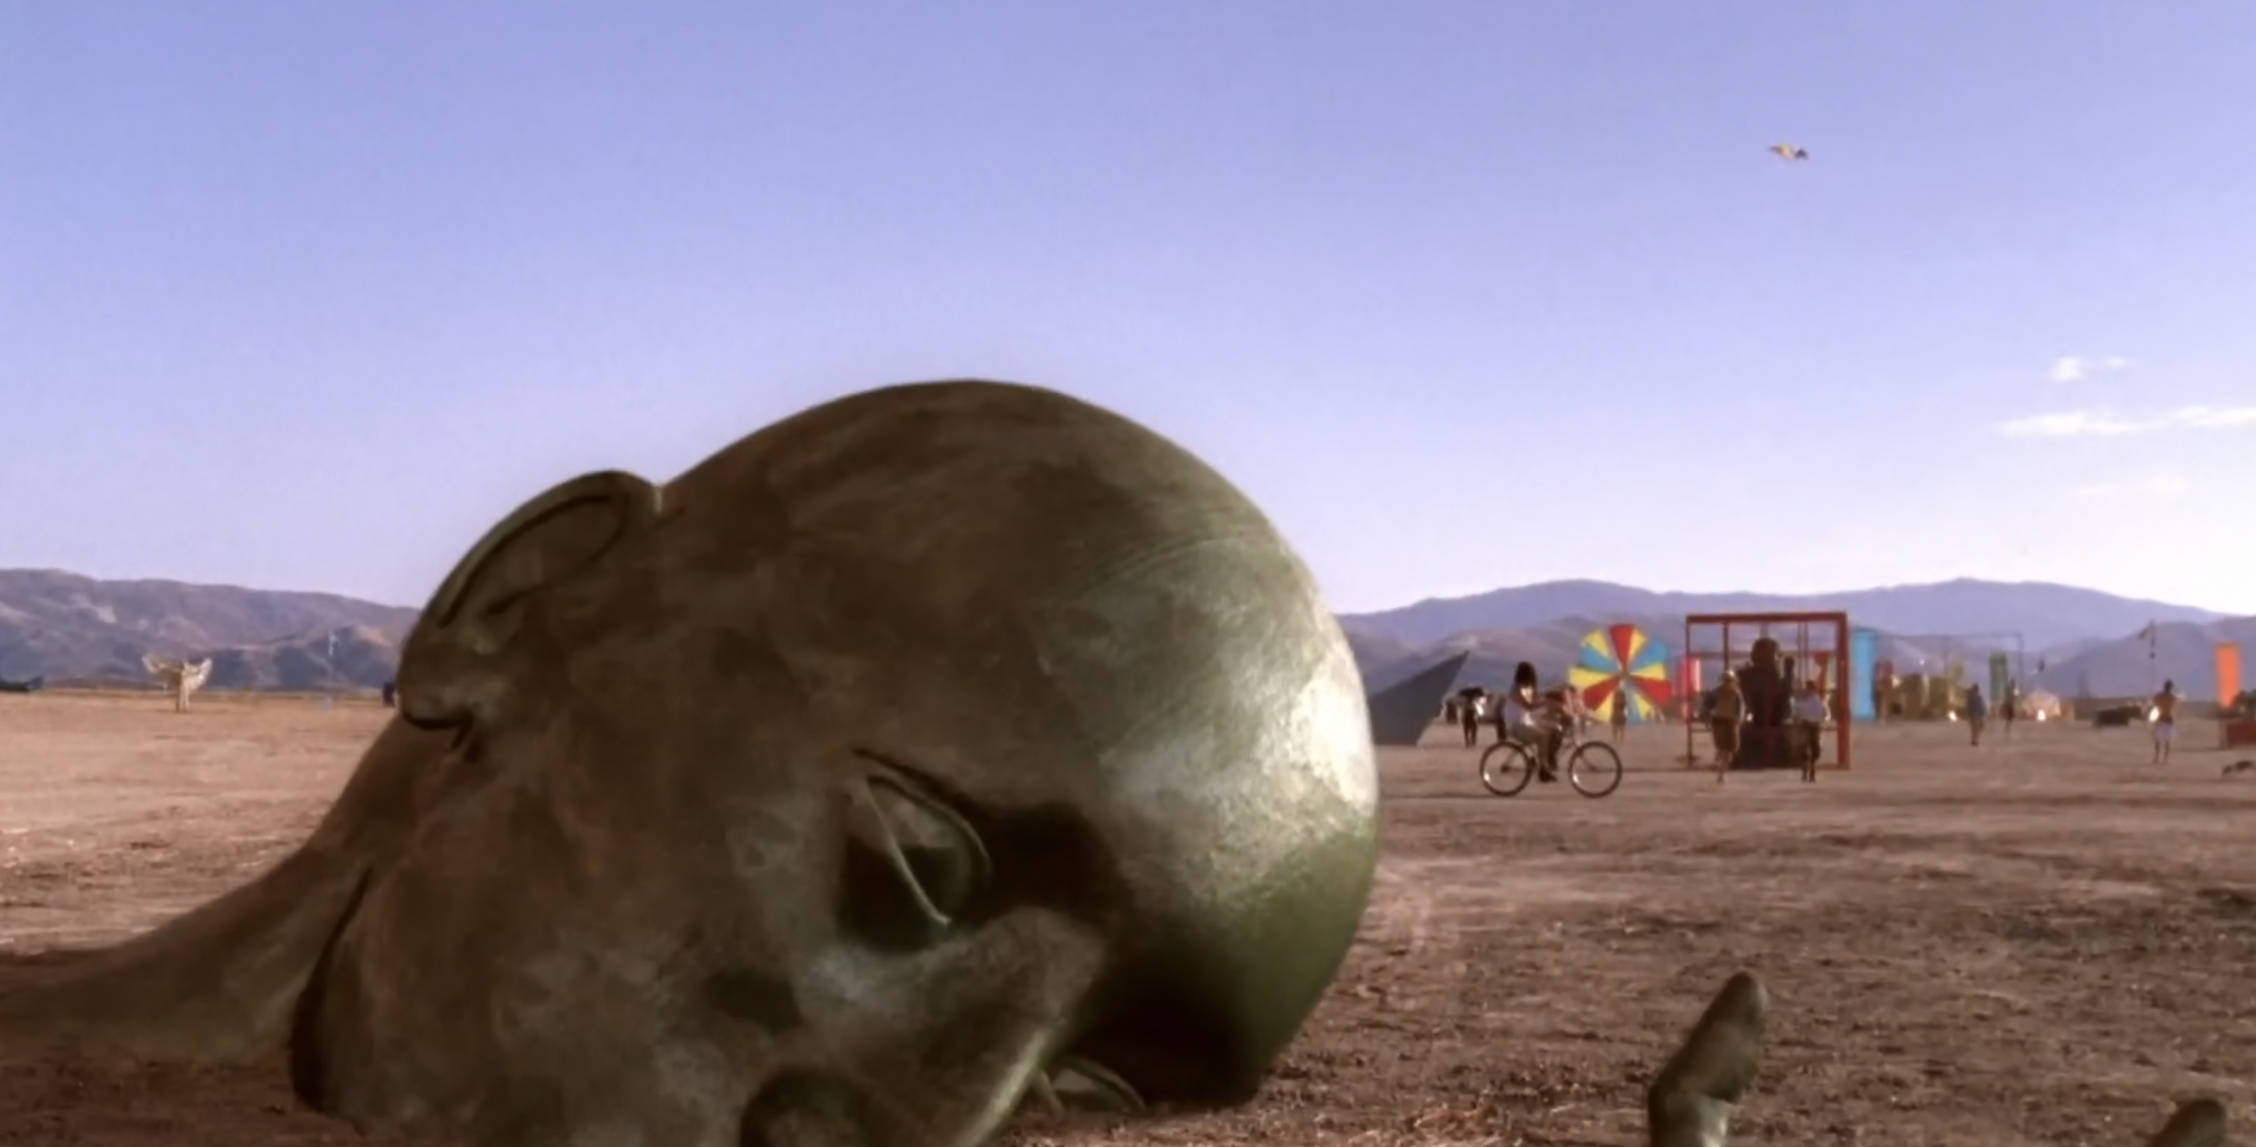
\includegraphics[width = 56.7mm, height=30mm]{images/malcolm1.png}
    \end{minipage}
    \vspace{\baselineskip}
    \begin{minipage}{.3\textwidth}
      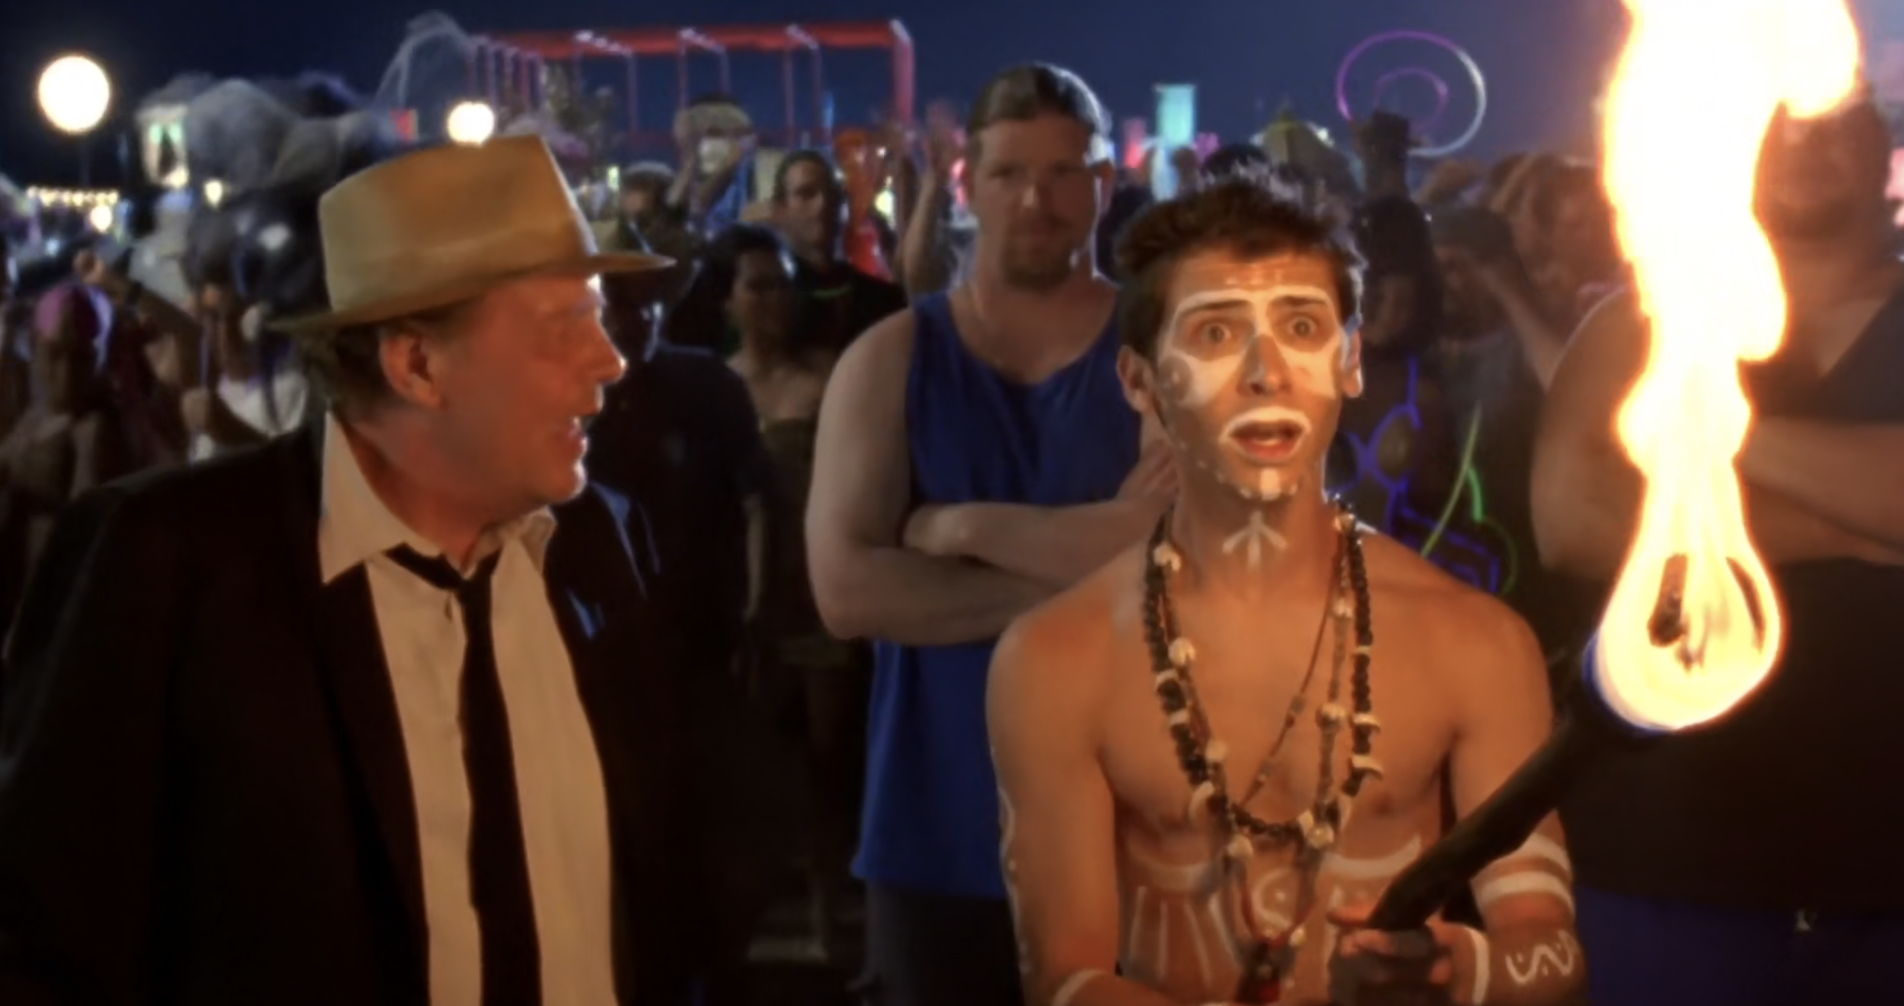
\includegraphics[height=30mm]{images/malcolm2.jpg}
    \end{minipage}
    \\
    \hline
  \end{tabular}
  \caption{Кадры}
  \label{table:2}
\end{table}

\subsection{Интересные формулы, всплывающие в фильмах}
Уравнение Шрёдингера в инвариантной форме имеет вид:\\
\[ \sum_{k,j} \Bigl[ -\frac{\hbar^2}{\sqrt{a}} \frac{\partial}{\partial q^k} \left( \sqrt{a}{a^k}^j \frac{\partial}{\partial q^j} \right) + V \Bigr]\Psi + \frac{\hbar}{i}\frac{\partial \Psi}{\partial t} = 0 \] \\
Уравнение Дирака (для свободной частицы):\\
\[i\hbar \frac{d\psi}{d t} = \Bigl[ c \sum_{i = 1}^3 \alpha_{i} p_{i} + \alpha_{0}m c^2\Bigr]\psi\]\\
Компоненты тензора Дарбу $\Theta$ вычисляются по формулам:\\
\[\Theta_{i j m} = \nabla_{m} b_{i j} - \frac{b_{i j}\nabla_{m}K + b_{mi}\nabla_{j}K + b_{j m}\nabla_{i}K}{4K}, i, j, m = 1, 2\]\\
Решения уравнения Бюргерса сводятся к положительным решениям линейного уравнения теплопроводности:\\
\[u(x, t) = 2\frac{\partial}{\partial x} \ln \left \{ (4\pi t)^{-\frac{1}{2}}\int_{-\infty}^\infty \exp \Bigl[ -\frac{(x - x^\prime)^2}{4t} - \frac{1}{2}\int_0^{x^\prime}u(x'', 0)dx''\Bigr]d x^\prime\right \}\]

\chapter{Заключение}

\begin{multicols}{2}
В данном исследовании необходимо было сравнить образы «Burning
Man» и ответить на ключевой вопрос «Как менялось представление
образа фестиваля «Burning Man» в произведениях массовой культуры
с 1995 по 2017 года?»

\begin{wrapfigure}{l}{0.5\linewidth}

\includegraphics[width=\linewidth]{images/signbm.jpg}
\caption{This is the Burning Man logo}
\end{wrapfigure}

В качестве~\cite{тихомирова2016фестиваль} теоретической составляющей были
изучены история фестиваля «Burning Man» и основные механизмы,
использующиеся в контент-аналитическом методе.


В ходе исследования были подробно изучены такие материалы как,
мультипликационный сериал «Симпсоны» (1995), сериал «Малкольм в
центре внимания» (2005), рассказ «Тусовщик» автора Чака Паланика
(2015), компьютерная игра «Watch Dogs 2» (2016) и художественный
фильм «Девушка из песни» (2017). Были получены результаты
сравнения образов фестиваля «Burning Man».

Таким образом, данное исследование показало, что неотъемлемой
частью образа «Burning Man» являлась его культура – церемония
сожжения и искусство, включающее в себя инсталляции, музыку,
танцы и костюмы участников. Передвижение по пустыне также
невозможно было представить без двухколесного транспортного
средства.

Изменения заключались в том, что в течение лет образ фестиваля
все сильнее связывали с внешним миром, и он все больше
противоречил десяти основным принципам, формирующимся на
протяжении всей истории «Burning Man». С 2015 года в образ
фестиваля стал входить алкоголь, а деньги приобрели свою 
ценность~\cite{фасмер1964этимологический}.
\end{multicols}

\printbibliography
\addcontentsline{toc}{chapter}{Список литературы}

\end{document}